% ------------------------------------------------------------------------------
% TYPO3 Version 10 LTS - What's New (French Version)
%
% @license	Creative Commons BY-NC-SA 3.0
% @link		https://typo3.org/help/documentation/whats-new/
% @language	French
% ------------------------------------------------------------------------------

\section{Tableau de bord}
\begin{frame}[fragile]
	\frametitle{Tableau de bord}

	\begin{center}\huge{\color{typo3darkgrey}\textbf{Tableau de bord}}\end{center}
	\begin{center}\large{\textit{Informations système, actualités et plus pour les utilisateurs backend}}\end{center}

\end{frame}

% ------------------------------------------------------------------------------
% Feature | 90333 | Dashboard

\begin{frame}[fragile]
	\frametitle{Tableau de bord}
	\framesubtitle{Vue backend (1)}

	Le tableau de bord est introduit pour afficher des informations système importantes à l'utilisateur backend authentifié.

	\begin{figure}
		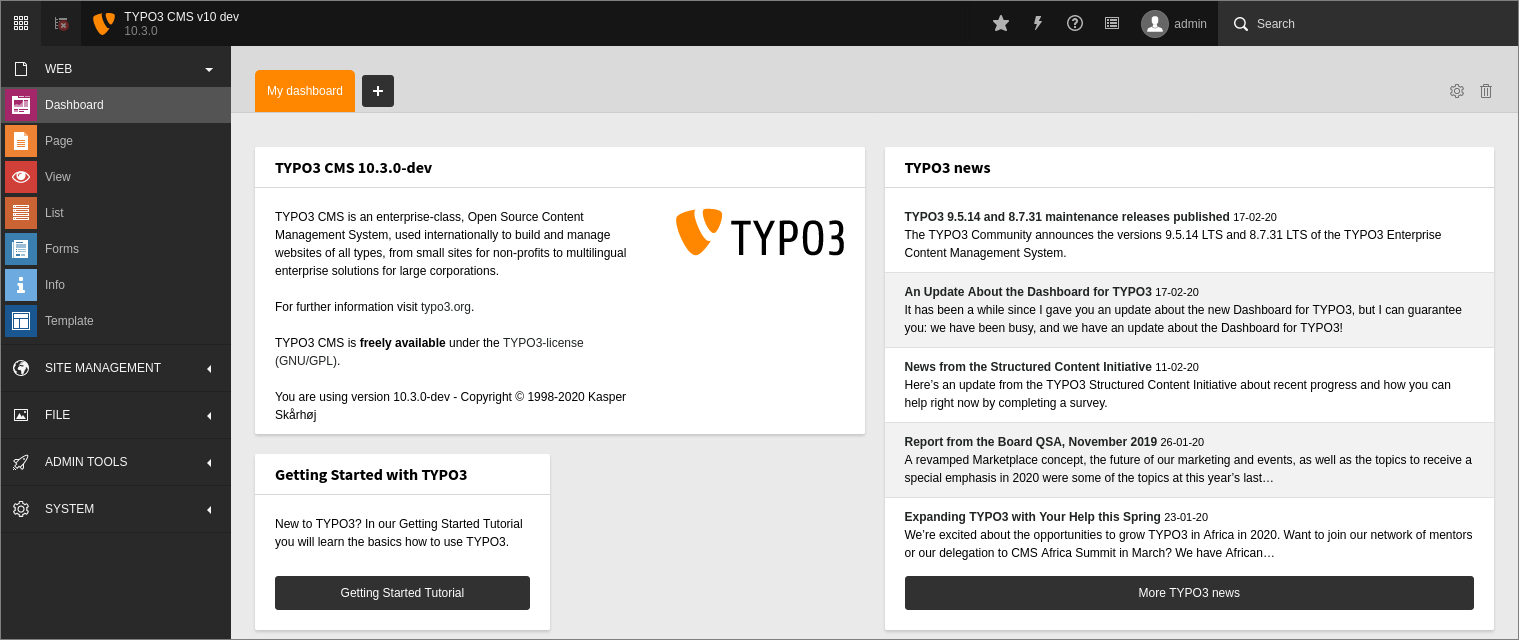
\includegraphics[width=0.9\linewidth]{Dashboard/90333a-Dashboard.png}
	\end{figure}

\end{frame}

% ------------------------------------------------------------------------------
% Feature | 90333 | Dashboard

\begin{frame}[fragile]
	\frametitle{Tableau de bord}
	\framesubtitle{Vue backend (2)}

	Les utilisateurs peuvent créer leurs propres tableaux de bord et personnaliser les widgets qui
	y sont placés.

	\begin{figure}
		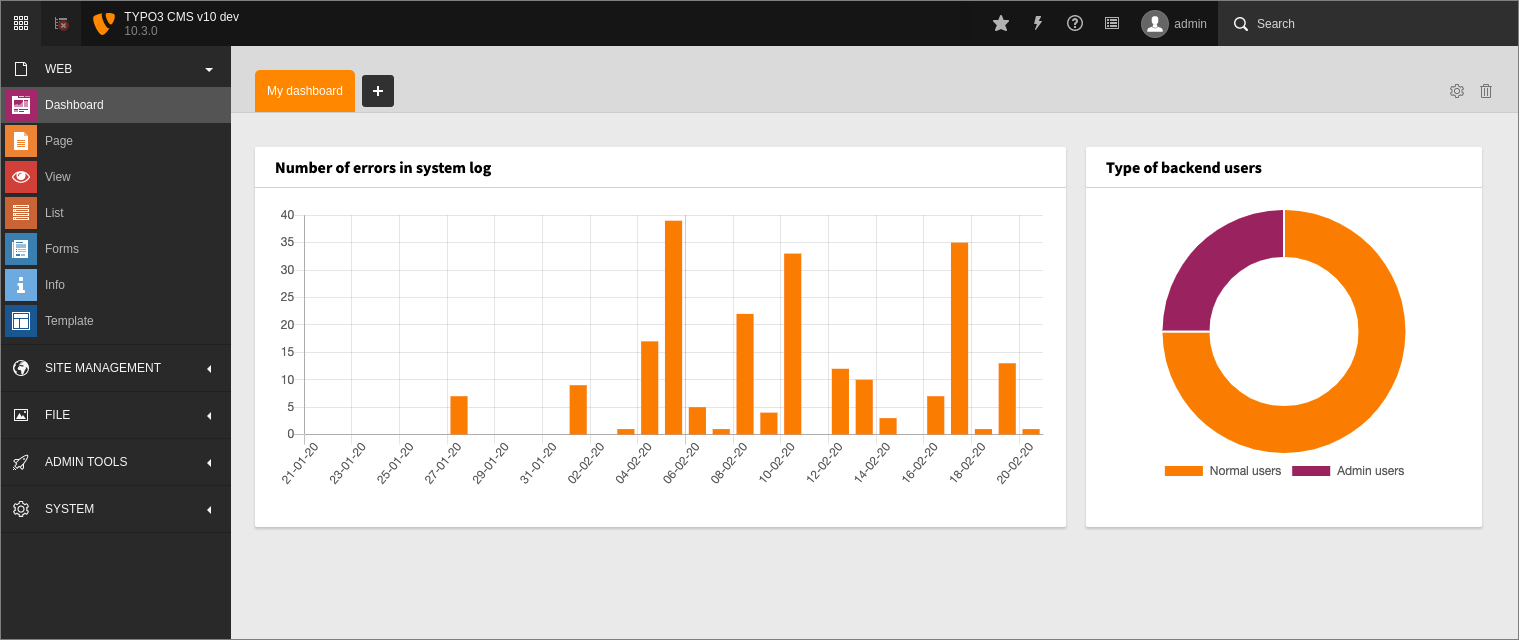
\includegraphics[width=0.9\linewidth]{Dashboard/90333b-Dashboard.png}
	\end{figure}

\end{frame}

% ------------------------------------------------------------------------------
% Feature | 90333 | Dashboard

\begin{frame}[fragile]
	\frametitle{Tableau de bord}
	\framesubtitle{Options pour les intégrateurs}

	% decrease font size for code listing
	\lstset{basicstyle=\tiny\ttfamily}

	\begin{itemize}
		\item Des tableaux de bord \textit{prédéfinis} peuvent être configurés pour les nouveaux utilisateurs et ceux qui n'en ont plus de défini.
		\item Un des usages est l'affichage d'un tableau de bord «~Démarrage~» par défaut.
		\item Exemple TSconfig~:

\vspace{-0.4cm}
\begin{lstlisting}
options.dashboard.dashboardPresetsForNewUsers = default, dashboardPreset-myPreset
\end{lstlisting}

		\item De multiples tableau de bord prédéfinis peuvent être indiqués sous
		forme de liste à virgule.
	\end{itemize}

\end{frame}

% ------------------------------------------------------------------------------
% Feature | 90333 | Dashboard

\begin{frame}[fragile]
	\frametitle{Tableau de bord}
	\framesubtitle{Widgets personnalisés}

	\begin{itemize}
		\item TYPO3 v10 LTS fournit quelques widgets de base\newline
			\smaller
				(par exemple~: informations générales, authentifications backend échouées, actualités TYPO3,
				liens de documentation, etc.)
			\normalsize
		\item Les développeurs peuvent créer des widgets dans leurs extensions.
		\item Inscription et configuration des widgets dans un fichier YAML~:\newline
			\small
				\texttt{EXT:myextension/Configuration/Services.yaml}
			\normalsize
		\item L'extension système "Dashboard" fourni des types de widget typiques\newline
			\smaller
				(histogramme, bouton d'action, graphique en anneaux, liste, nombre et icônes, et rss)
			\normalsize
		\item Pour en savoir plus, consultez la
			\href{https://docs.typo3.org/c/typo3/cms-dashboard/master/en-us/}{documentation TYPO3 (en)}.

	\end{itemize}

\end{frame}

% ------------------------------------------------------------------------------
